\saltoPag{}
\section{UNIDAD 3}
    \subsection{Postulados de la teoría de Lewis}
        \begin{enumerate}
            \item Los electrones ($e^-$) de valencia participan en el enlace químico.
            \item En algunos casos se transfieren ($e^-$) de un átomo a otro, formándose iones ($+$) y ($-$) que se atraen mediante fuerzas electrostáticas llamadas ''Enlaces iónicos''.
            \item En otros se comparten uno o más pares de $e^-$, generando un enlace covalente.
            \item Los $e^-$ se transfieren o comparten de manera que los átomos adquieren una configuración estable. En general es una configuración de gas noble con 8 $e^-$ de valencia que constituyen un octeto.
        \end{enumerate}
        
        \sangria{} Los electrones de valencia son los últimos electrones de un orbital en un átomo, que son los causantes de los enlaces químicos.
        \begin{center} 
            \begin{tabular}{| c | c | c |}
                \toprule
                \textbf{Grupo} & \textbf{$e^-$ configuración} & \textbf{$N^o e^-$ de valencia} \\ 
                \midrule
                \midrule
                1A & $ns^\text{\textcolor{red}{\textbf{1}}}$ & 1 \\
                \midrule
                2A & $ns^\text{\textcolor{red}{\textbf{2}}}$ & 2 \\
                \midrule
                3A & $ns^\text{\textcolor{red}{\textbf{2}}}np^\text{\textcolor{red}{\textbf{1}}}$ & 3 \\
                \midrule
                4A & $ns^\text{\textcolor{red}{\textbf{2}}}np^\text{\textcolor{red}{\textbf{2}}}$ & 4 \\
                \midrule
                5A & $ns^\text{\textcolor{red}{\textbf{2}}}np^\text{\textcolor{red}{\textbf{3}}}$ & 5 \\
                \midrule
                6A & $ns^\text{\textcolor{red}{\textbf{2}}}np^\text{\textcolor{red}{\textbf{4}}}$ & 6 \\
                \midrule
                7A & $ns^\text{\textcolor{red}{\textbf{2}}}np^\text{\textcolor{red}{\textbf{5}}}$ & 7 \\
                \bottomrule
            \end{tabular}
        \end{center}

        \begin{center} \textcolor{blue}{\underline{Estructura de Lewis para los elementos } \\ \underline{representativos y gases nobles}} \end{center}
        \begin{center} 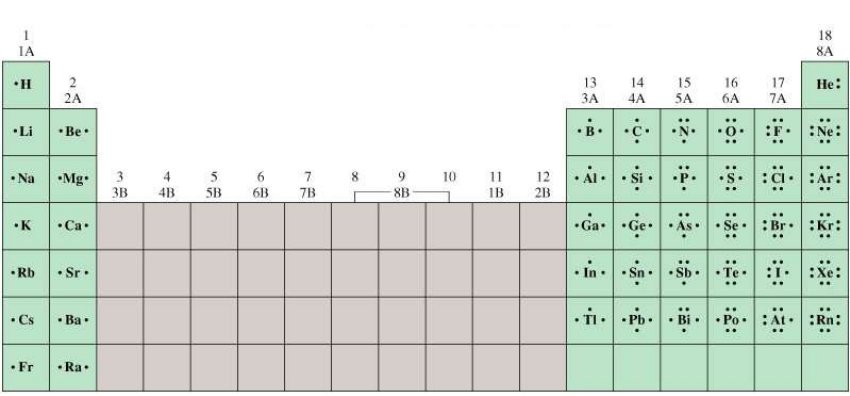
\includegraphics[width=8cm]{./imagenes/estructuraLewisElementosReprenYGasesNobles.png} \end{center}

    \subsection{Enlace iónico}
        \sangria{} Resulta de las interacciones electrostáticas entre iones. Hay una transferencia de electrones de un átomo a otro.
        \begin{center} 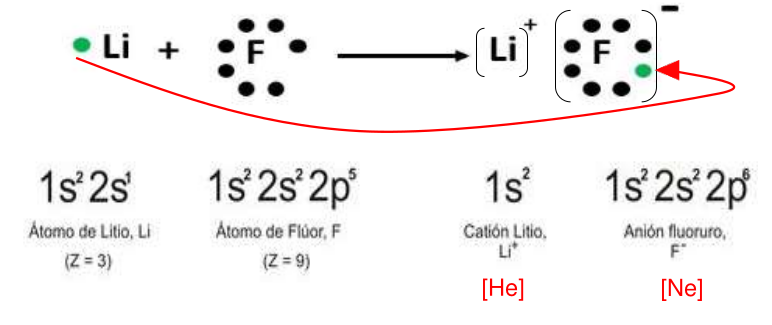
\includegraphics[width=6cm]{./imagenes/ejemploEnlaceIonico.png} \end{center} \columnbreak{}

        \begin{center} \textcolor{red}{\underline{Estabilidad de los compuestos iónicos}} \end{center}

        \sangria{} Para poder medir la ''estabilidad'' de un compuesto iónico se puede usar la energía reticular, que es aquella necesaria para separar completamente un mol de un compuesto sólido en sus iones gaseosos. Véase la ley de Coulomb:

        \begin{center} $E = k\frac{Q^+Q^-}{r}$ \end{center}

        \sangria{} Siendo:
        \begin{itemize} 
            \item $Q^+$: carga del catión.
            \item $Q^-$: carga de anión.
            \item $r$: distancia entre ambos.
        \end{itemize}

        \sangria{} Ejemplos:
        \begin{center}
            \begin{tabular}{| c | c |}
                \toprule
                \textbf{Compuesto} & \textbf{Energía de separación} \\
                \midrule
                \midrule
                $MgF_2$ & $2957 Q = +2, -1$ \\
                \midrule
                $MgO$ & $3928 Q= +2, -2$ \\
                \midrule
                $LiF$ & $1036 rF^- < r Cl^-$ \\
                \midrule
                $LiCl$ & $853 rF^- < r Cl^-$ \\
                \bottomrule
            \end{tabular} \\[1cm]
        \end{center} 
        \begin{center} \textcolor{red}{\textbf{Ciclo de Born-Haber para determinar la energía reticular}} \\ 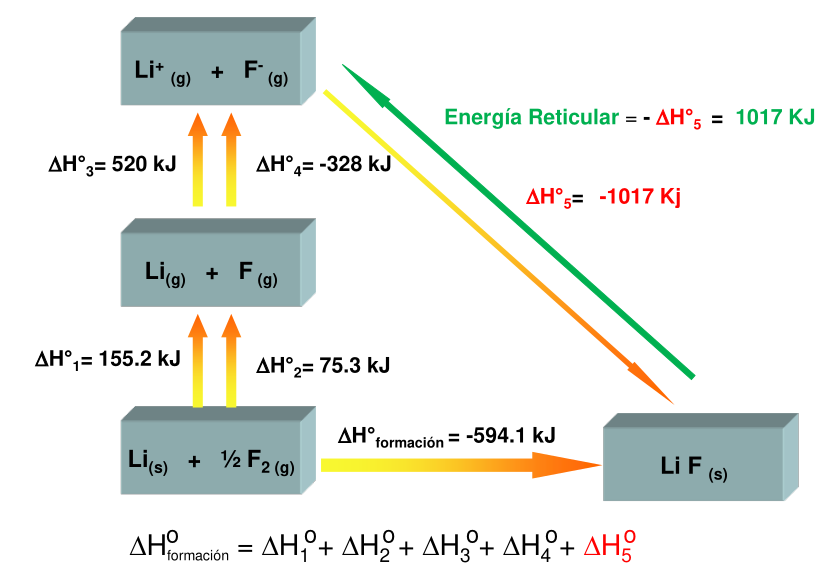
\includegraphics[width=8cm]{./imagenes/cicloBornHaberEnergiaReticular.png} \end{center}
        \begin{center} \textcolor{red}{\textbf{Ejemplos de algunos valores de energía reticular}} \\ 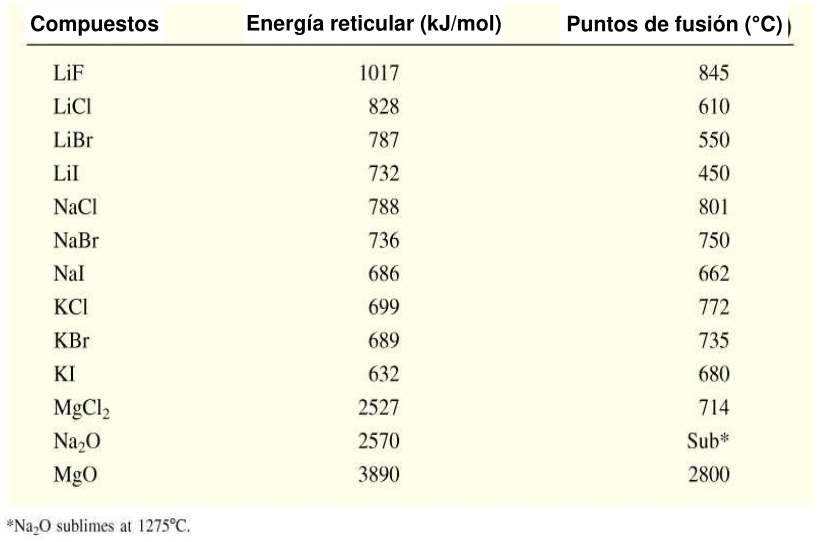
\includegraphics[width=8cm]{./imagenes/ejemplosEnergiaReticular.png} \end{center}
    \saltoPag{}
    \subsection{Enlace covalente}
        \sangria{} Resulta de compartir un par de electrones entre dos átomos. Se trata de alcanzar el mismo número de electrones en la capa de valencia que los gases nobles más cercanos a ellos en la tabla periódica (regla del octeto).
        \begin{center} \textbf{Estructura de Lewis} \end{center}
        \begin{enumerate} 
            \item Elegir un esqueleto simétrico.
            \item Dibuje la estructura del compuesto mostrando qué átomos están conectados con otros. Coloque ele elemento menos electronegativo al centro.
            \item Los átomos de oxígeno no se enlazan entre sí, salvo en $O_2$ y $O_3$, los peróxidos y superóxidos.
            \item El hidrógeno y el flúor ocupan posiciones terminales.
            \item Calcule el número total de electrones de valencia. Agregue 1 por cada carga negativa y elimine 1 por cada carga positiva.
            \item Complete los octetos de electrones para todos los elementos, excepto para el $H(2e^-), Be(4e^-), Al y B(6e^-)$.
            \item Forme enlaces dobles o triples en el átomo central cuando sea necesario.
        \end{enumerate}

        \begin{center} \textbf{\underline{Ejemplo:}} \textit{Estructura de Lewis para el $CCl_4$} \end{center}
        \begin{enumerate} 
            \item El $C$ es el átomo central ya que es menos electronegativo que el $Cl$. 
            \item Contar los electrones necesarios ($N$) para completar el octeto (teniendo en cuenta las excepciones de esta regla).
                \begin{center} 
                    $C = 8 e^-$ \\[5pt]
                    $Cl = 8 e^-$ \\[5pt]
                    \textcolor{red}{\textbf{$N$}} $= 8 + (4 \times 8) = $ \textcolor{red}{\textbf{40 electrones necesarios}}
                \end{center}
            \item Contar los electrones disponibles ($D$) de valencia que forman parte de la estructura (agregar o quitar tantas unidades como carga negativas o positivas tenga el compuesto).
                \begin{center} 
                    $C = e^-$ de valencia, configuración externa $= 2s^2 2p^2$ \\[10pt]
                    $Cl = 7 e^-$  de valencia, configuración externa $= 3s^2 3p^5$ \\[10pt]
                    \textcolor{red}{\textbf{$D$}} = $4 + (4 \times 7) =$ \textcolor{red}{\textbf{32 electrones de valencia disponibles}}
                \end{center}

            \item Calcular los $e^-$ compartidos:
                \begin{center}
                    $C = N - D$ \\[5pt]
                    $C = 40 - 32$ \\[5pt]
                    $C =$ \textcolor{red}{\textbf{8 $e^-$ compartidos, 4 enlaces.}}
                \end{center}
            \item Dibujar enlaces imples entre los átomos de $C$ y $Cl$ completando los octetos:
                \begin{center} 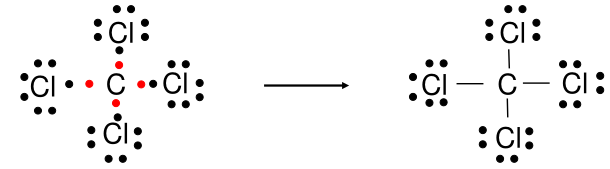
\includegraphics[width=8cm]{./imagenes/dibujoLewisCCl4.png} \end{center}
                \sangria{} Nótese que:
                    \begin{enumerate}
                        \item Hay un \textbf{enlace simple} (dos átomos comparten un par de $e^-$).
                        \item Los puntos negros ($e^-$) son pares de electrones no compartidos.
                    \end{enumerate}
        \end{enumerate}

    \subsection{Electro-negatividad}
        \sangria{} La electro-negatividad es la capacidad de un átomo para atraer los electrones de otro átomo en un enlace químico. \\
        \sangria{} El tipo de enlace estará dado en relación a la diferencia de electro-negatividad entre los átomos que forman el compuesto. \\
        \sangria{} El enlace polar es un enlace covalente donde la diferencia de electro-negatividad entre los dos átomos no es muy grande (aproximadamente menos a 2).
        \begin{center} \textcolor{red}{\underline{Distorsión de la nube electrónica entre} \\ \underline{dos átomos con diferente electro-negatividad}} \\[10pt] 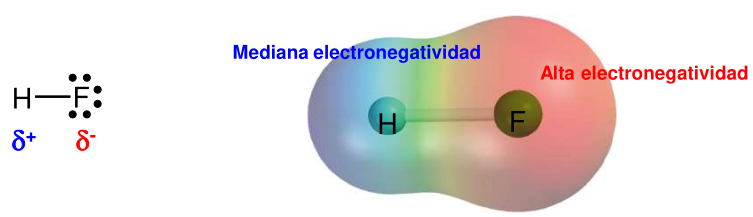
\includegraphics[width=8cm]{./imagenes/distorsionNubeElectronicaEntreAtomosDiferenteElectroNeg.png} \\[10pt] \textit{Electro-negatividad es relativa, $F$ es el más electro-negativo que el $H$} \end{center}
        \begin{center} \textcolor{red}{\underline{Clasificación de los enlaces por electro-negatividad}} \end{center}
        \sangria{} El tipo de enlace estará dado en relación a la diferencia de electro-negatividad entre los átomos que forman el compuesto.
        \begin{center} 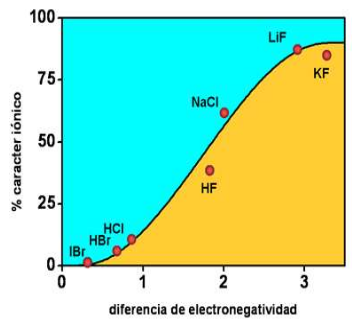
\includegraphics[width=4cm]{./imagenes/clasificacionEnlacesElectronegatividad.png} \end{center}
        \begin{center}
            \begin{tabular}{| c | c |}
                \toprule
                \textbf{Diferencia} & \textbf{Tipo de enlace} \\
                \midrule
                0 & Covalente \\
                \midrule
                $\geq 2$ & Iónico \\
                \midrule
                $0 < y < 2$ & Covalente Polar \\
                \bottomrule
            \end{tabular}
        \end{center}
        \saltoPag{}
        \begin{center} 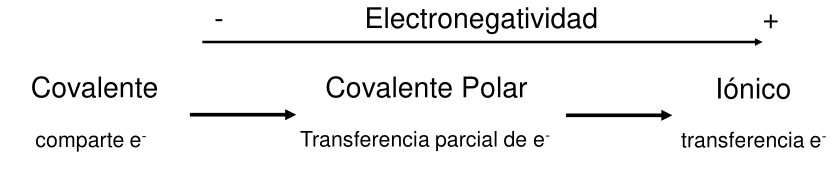
\includegraphics[width=8cm]{./imagenes/evolucionElectronegatividad.png} \end{center}

        \begin{center} \textcolor{red}{\underline{Electro-negatividades en la tabla periódica}} \\[5pt] 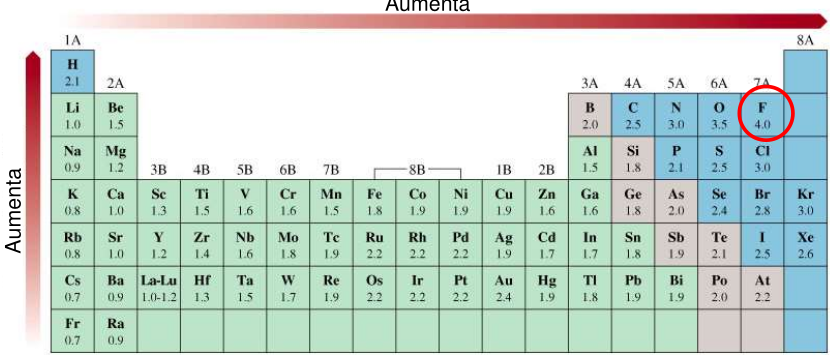
\includegraphics[width=8cm]{./imagenes/electronegatividadesEnLaTablaPeriodica.png} \end{center}

        \begin{center} \textcolor{red}{\underline{Longitud de los enlaces covalente}} \end{center}
        \begin{center} 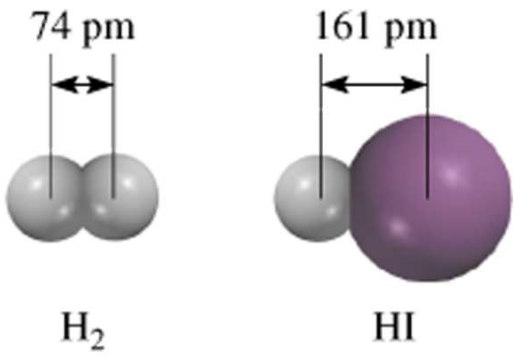
\includegraphics[width=4cm]{./imagenes/longitudEnlCovalenteH2yHI.png} 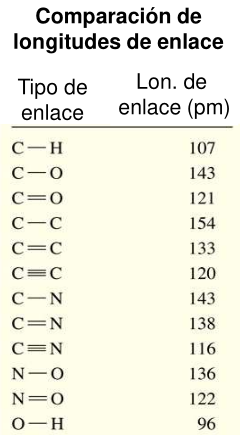
\includegraphics[width=3cm]{./imagenes/comparacionDeLongitudesDeEnlace.png} \end{center}
        \begin{center} 
            \begin{tabular}{| c |}
                \toprule
                \textbf{Longitud} \\
                \midrule
                Triple enlace $<$ Doble enlace $<$ Enlace simple \\
                \bottomrule
            \end{tabular}
        \end{center}
        \begin{center} \textcolor{red}{\underline{Energía de enlace}} \end{center}
        \sangria{} Es el cambio necesario en la entalpía para romper un enlace de un mol de un compuesto gaseoso.
        \begin{center}
            \begin{tabular}{| c |}
                \toprule
                \textbf{Energía de enlace} \\
                \bottomrule
            \end{tabular}
            \begin{tabular}{| c | c |}
                \toprule
                $H_{2(g)} \rightarrow H_{(g)} + H_{(g)}$ & $\Delta H^0 = 436,4 kJ$ \\
                \midrule
                $Cl_{2(g) \rightarrow Cl_{(g)} + Cl_{(g)}}$ & $\Delta H^0 = 242,7 kJ$ \\
                \midrule
                $HCl_{(g) \rightarrow H_{(g) + Cl_{(g)}}}$ & $\Delta H^0 = 431,9 kJ$ \\
                \midrule
                $O_{2(g) \rightarrow 0_{(g) + O_{(g)}}}$ & $\Delta H^0 = 498,7 kJ$ 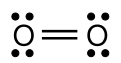
\includegraphics[width=10mm]{./imagenes/diagramaLewisO2.png} \\
                \midrule
                $N_{2(g) \rightarrow N_{(g) + N_{(g)}}}$ & $\Delta H^0 = 941,4 kJ$ 
\includegraphics[width=10mm]{./imagenes/diagramaLewisH2.png} \\
                \bottomrule
            \end{tabular} \\[1cm]
            \begin{tabular}{| c |}
                \toprule
                \textbf{Energía de enlace} \\
                \midrule
                Enlace sencillo $<$ Enlace doble $<$ Enlace triple \\
                \bottomrule
            \end{tabular}
        \end{center}

        \begin{center} \textcolor{red}{\underline{Estructura resonante}} \end{center}
        \sangria{} Ocurre cuando dos o más estructuras de Lewis para una misma molécula no pueden ser representadas gráficamente por una sola estructura de Lewis. 
        \columnbreak{}
        \begin{center} \textbf{\underline{Ejemplo:}} \textit{estructura de Lewis para el anión ${NO_3}^{-}$} \end{center}
        \begin{center}
            $C = N -D$ \\
            $C = (8 + 8 \times 3) - (5 + 6 \times 3 + 1)$ \\
            $C = 32 - 24$ \\
            $C =$ \textcolor{red}{\textbf{8 $e^-$ compartidos y 4 enlaces}}
        \end{center}
        \sangria{} Se resta un electrón por cada carga positiva y se sumó un electrón por cada carga negativa.
        \begin{center} 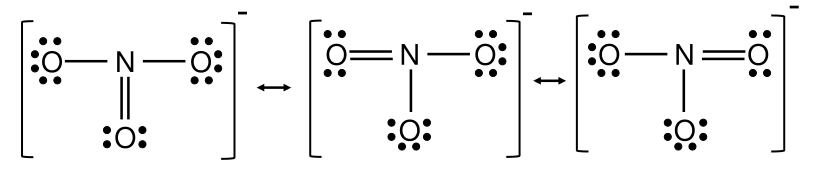
\includegraphics[width=8cm]{./imagenes/estructuraResonanteNO3-.png} \end{center}

        \begin{center} \textcolor{red}{\underline{Resumen}} \end{center}
        \begin{itemize}
            \item Los enlaces químicos son las fuerzas que mantienen unidos a los átomos en las moléculas de los elementos ($0_2$ y $Cl_2$); de compuestos ($CO_2$ y $H_2O$) y de metales.
            \item Los átomos se combinan con el fin de alcanzar una configuración electrónica más estable.
            \item La estabilidad máxima se produce cuando un átomo es iso-electrónico con un gas noble.
            \item Solo los electrones externos de un átomo pueden ser atraídos por otro átomo cercano.
            \item En la formación de enlaces químicos solo intervienen los electrones de valencia.
        \end{itemize}
    \longsubsection{Teoría de repulsión de los pares electrónicos de la capa de valencia}{Teoría de repulsión de los pares electrónicos de la capa de valencia}
    \sangria{} Predicción de la geometría de las moléculas mediante la repulsión electrostática de pares de electrones compartidos y no compartidos. \\[10pt]
    \sangria{} \textbf{\underline{Grupo electrónico:}} enlace simple, doble o triple ó un par de electrones no enlazados. \\[10pt]
        \begin{center}
            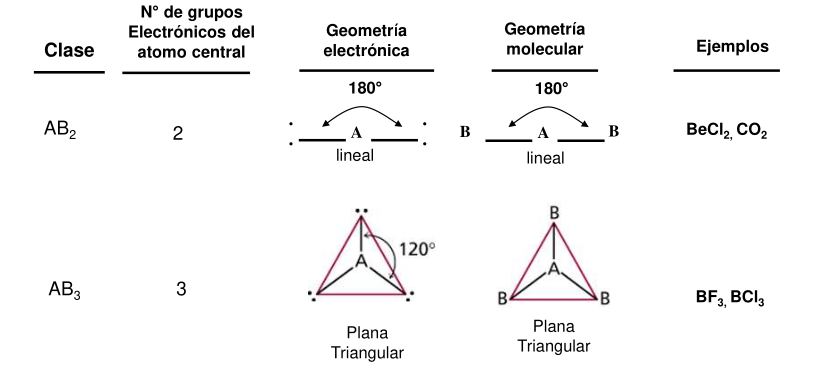
\includegraphics[width=7cm]{./imagenes/geometriaElectronica1.png}
            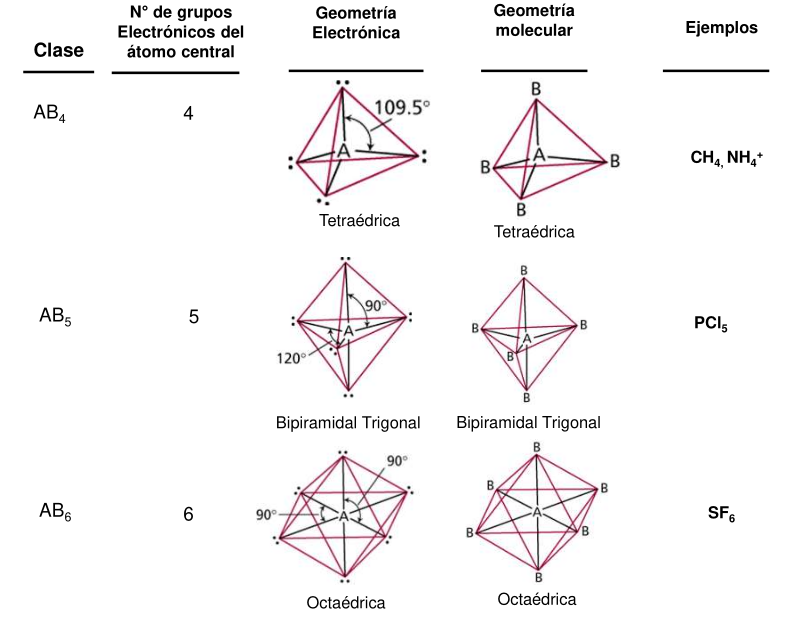
\includegraphics[width=7cm]{./imagenes/geometriaElectronica2.png}
        \end{center}
        \saltoPag%
        \begin{center}
            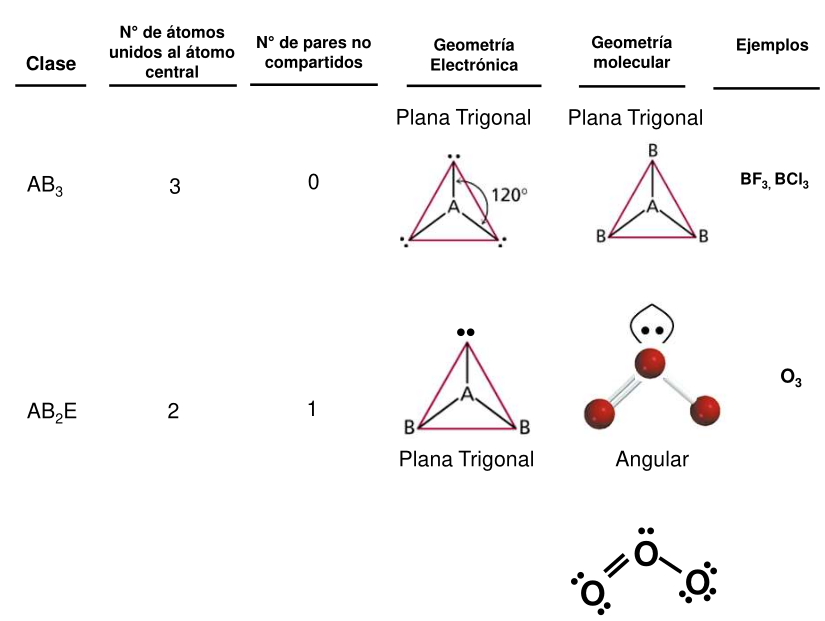
\includegraphics[width=7cm]{./imagenes/geometriaElectronica3.png}
            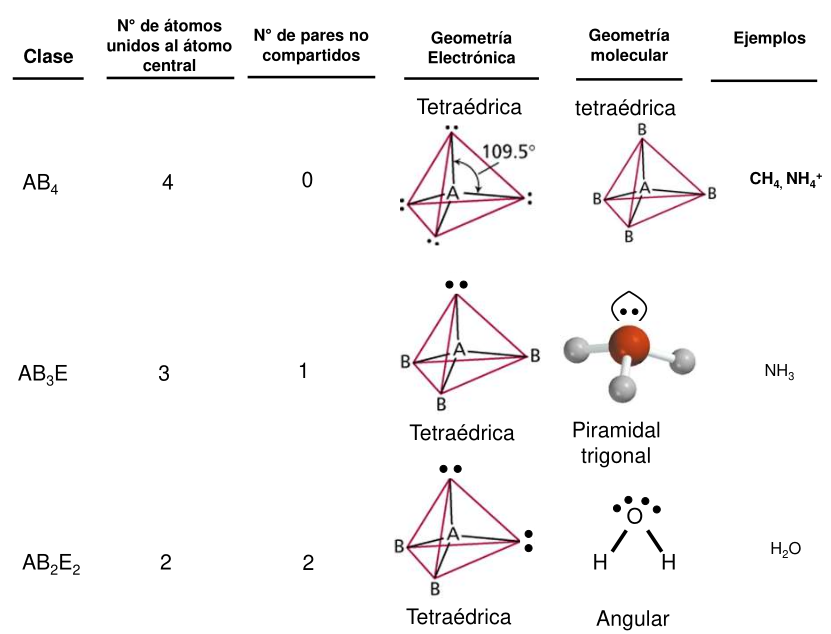
\includegraphics[width=7cm]{./imagenes/geometriaElectronica4.png}
        \end{center}
    \longsubsection{Repulsión de pares de electrones}{Repulsión de pares de electrones}
        \begin{center} 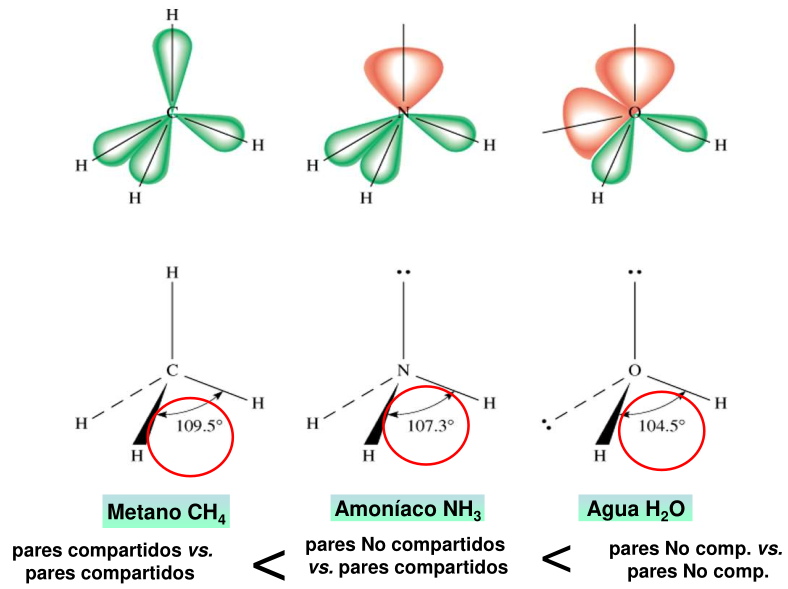
\includegraphics[width=7cm]{./imagenes/ejemplosRepulsionParesElectrones.png} \end{center}
    \subsection{Momentos dipolares y moléculas polares} 
        \begin{center} 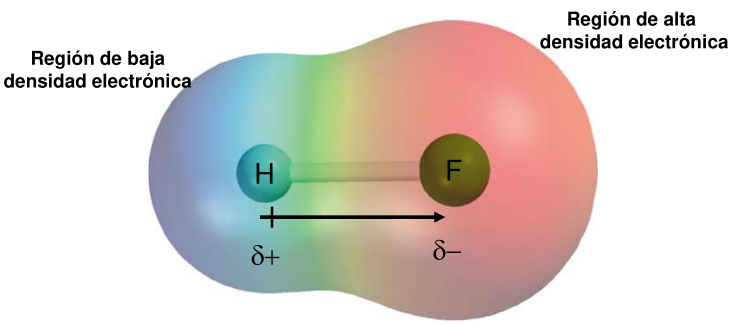
\includegraphics[width=6cm]{./imagenes/momentosDipolaresYMoleculasPolares.png} \end{center}
        \begin{center}
            \begin{tabular}{| c | c |}
                \toprule
                \textbf{Medida de polaridad} & \textbf{Expresión} \\
                \midrule
                $\mu = Q \cdot r$ & $Q$: producto de la carga($C$). \\& $r$: distancia($m$). \\
                \midrule
                \textbf{Valor en Debye ($D$)} & \textbf{Expresión} \\
                \midrule
                $1D$ & $3,36 \times 10^{-30}C \cdot m$ \\
                \midrule
            \end{tabular}
        \end{center}
        \columnbreak{}
        \begin{center}
            \begin{tabular}{| c |}
                \toprule
                \textbf{Valor de $\mu$ para moléculas no polares} \\
                \midrule
                $\mu = 0$ \\
                \bottomrule
            \end{tabular}
        \end{center}
    \subsection{Comportamiento de moléculas polares}
        \begin{center} 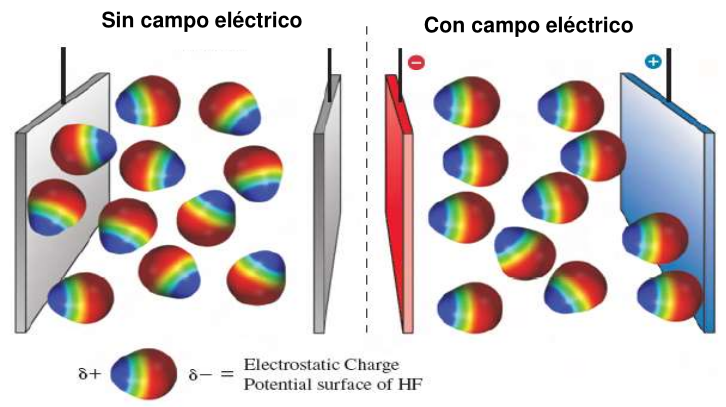
\includegraphics[width=7cm]{./imagenes/comportamientoMoleculasPolares.png} \end{center}
        \begin{center} \textcolor{red}{\underline{Otros ejemplos de momentos dipolares}} \end{center}
        \begin{center} 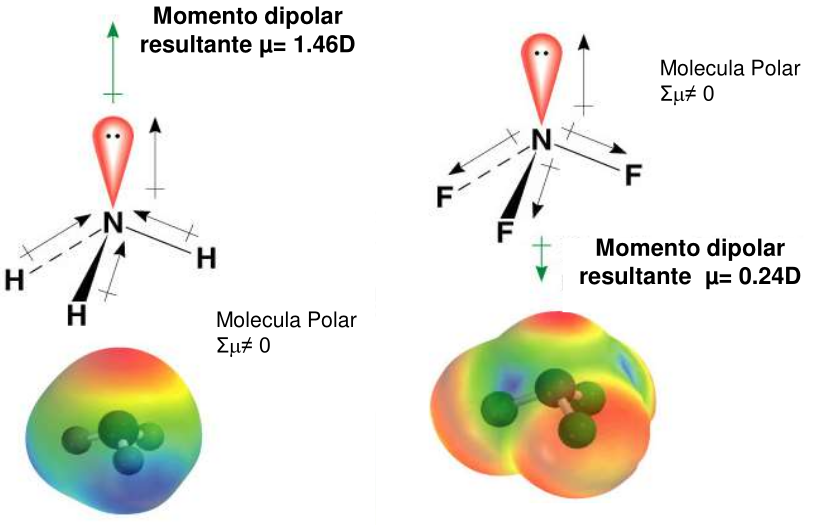
\includegraphics[width=7cm]{./imagenes/geometriaMomentoDipolar.png} \end{center}
        \sangria{} Moléculas polares:
        \begin{itemize} 
            \item El átomo central, en general, tiene pares de electrones no enlazantes.
            \item Su geometría es asimétrica.
        \end{itemize}
        \begin{center} \textcolor{red}{\underline{Momento dipolar ($\mu$) en la serie de halogenuros de hidrógeno}} \\[10pt] 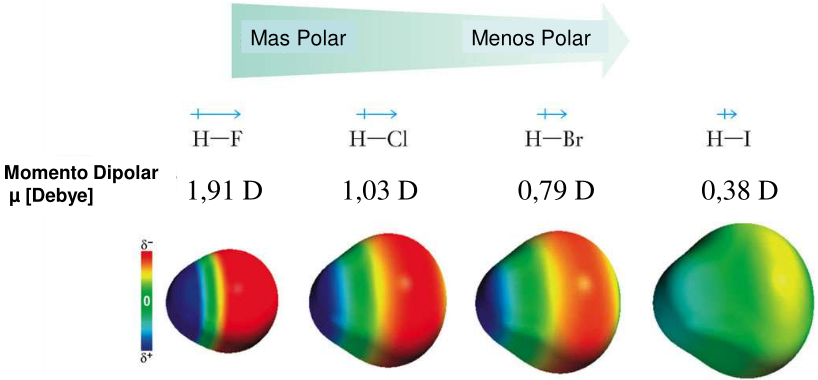
\includegraphics[width=8cm]{./imagenes/momentoDipolarHalogenurosHidrogeno.png} \end{center} 
        \textbf{\underline{Ejemplo:}} $CH_2F_2$ \textit{Molécula polar} \\[2mm] Siendo $\sum \mu \neq 0$
        \begin{center} 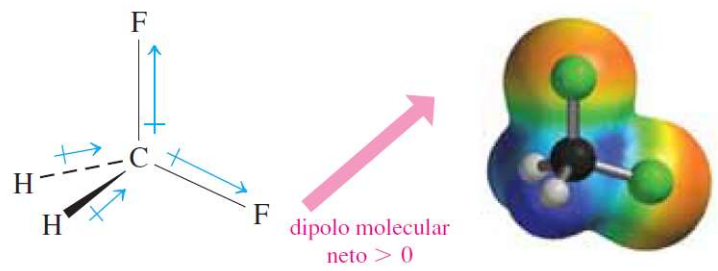
\includegraphics[width=7cm]{./imagenes/momentoDipolarCH2F2.png} \end{center}
        \saltoPag%
        \begin{center} \textcolor{red}{\underline{Moléculas \textbf{apolares} tienen un $\mu = 0$}} \end{center}
        \begin{center} 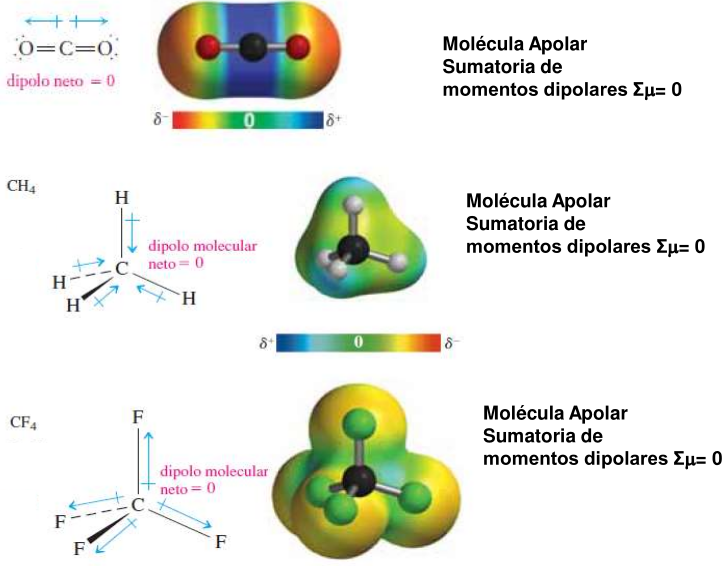
\includegraphics[width=7cm]{./imagenes/momentoDipolarMoleculasApolares.png} \end{center}
    \subsection{Enlaces sigma ($\sigma$) y Pi ($\pi$)}
        \begin{tabular}{| c | c |}
            \toprule 
            Enlace simple & 1 enlace $\sigma$ \\
            \midrule
            Enlace doble & 1 enlace $\sigma$ y 1 enlace $\pi$ \\
            \midrule
            Enlace triple & 1 enlace $\sigma$ y 2 enlaces $\pi$ \\
            \bottomrule
        \end{tabular}

        \subsubsection{Enlaces múltiples}
        \begin{center} \textcolor{red}{\textbf{\underline{Dobles}}} \\[5pt] 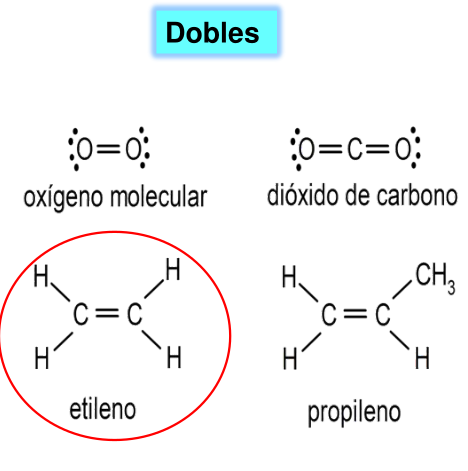
\includegraphics[width=3cm]{./imagenes/enlacesDobles.png} \\[10pt] \textcolor{red}{\textbf{\underline{Triples}}} \\[5pt] 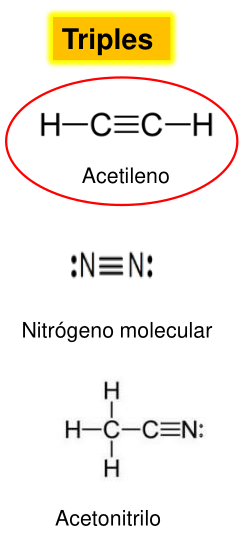
\includegraphics[width=3cm]{./imagenes/enlacesTriples.png} \end{center}

    \subsection{Teoría de los orbitales moleculares}
        \sangria{} Niveles de energía de enlace y de anti-enlace en el orbital molecular del hidrógeno ($H_2$).
        \begin{center} 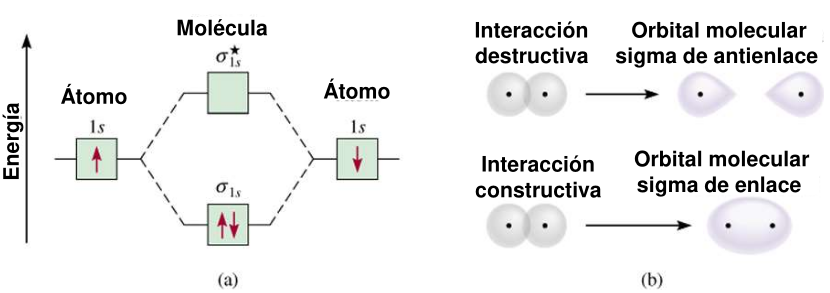
\includegraphics[width=8cm]{./imagenes/enlaceYAntiEnlace.png} \end{center}
        \sangria{} Un \textbf{orbital molecular de enlace} tiene menos energía y mayor estabilidad que los orbitales atómicos que lo formaron. \\
        \sangria{} Un \textbf{orbital molecular de anti-enlace} tiene más energía y menor estabilidad que los orbitales atómicos que lo formaron.
        \begin{center} \textcolor{red}{\underline{Interferencia constructiva y destructiva}\\ \underline{de dos ondas con la misma longitud y amplitud}} \\[10pt] 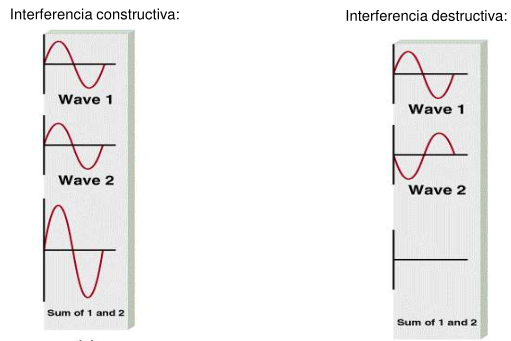
\includegraphics[width=8cm]{./imagenes/interferenciaConstructivaYDestructiva.png} \end{center}
        \begin{center} \textcolor{red}{\underline{Interacciones posibles entre dos orbitales} \\ \underline{equivalentes $p$}} \end{center}
        \begin{center}
            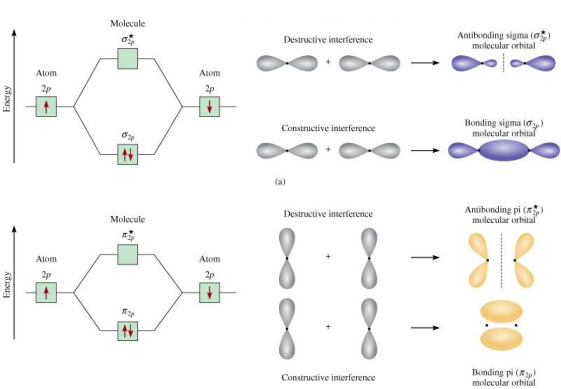
\includegraphics[width=7cm]{./imagenes/interaccionesPosiblesOrbitalesEqP1.png} \\[1cm]
            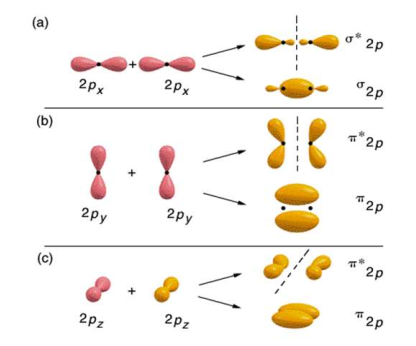
\includegraphics[width=7cm]{./imagenes/interaccionesPosiblesOrbitalesEqP2.png}
        \end{center}
        \saltoPag{}

    \subsection{Configuraciones de orbitales moleculares}
        \begin{itemize} 
            \item El número de O.M. que se forma siempre es igual al número de orbitales atómicos que se combinan.
            \item Cuanto más estable es el O.M. de enlace, menos estable es el O.M. del anti-enlace correspondiente.
            \item Los O.M. se llenan de acuerdo con su nivel de energía.
            \item Cada O.M. puede tener hasta dos electrones.
            \item Se utiliza la regla de Hund cuando se añaden electrones a los O.M. del mismo nivel de energía.
            \item El número de electrones en los O.M. es igual a la suma de todos los electrones en los átomos unidos.
        \end{itemize}
        \begin{center} Orden de enlace $= \frac{1}{2} (n - m)$ \end{center}
        Siendo:
        \begin{itemize}
            \item $n$: Número de electrones en los O.M. de enlaces.
            \item $m$: Número de electrones en los O.M. de anti-enlaces.
        \end{itemize}
        \begin{center} 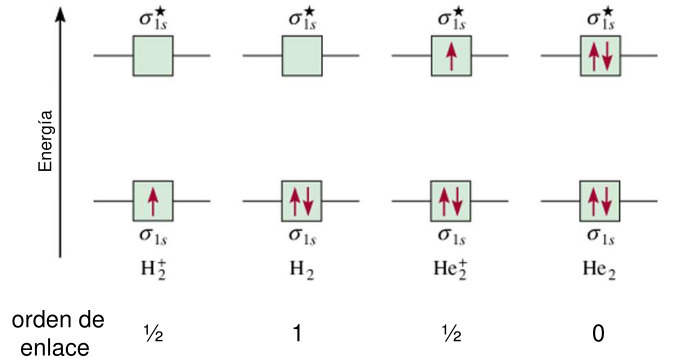
\includegraphics[width=8cm]{./imagenes/ordenDeEnlaces.png} \end{center}
    \subsection{Enlace metálico}
        \begin{center} 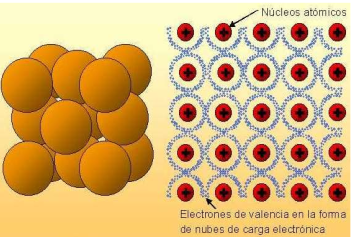
\includegraphics[width=5cm]{./imagenes/enlaceMetalico1.png} \end{center}
        \sangria{} Orbitales de valencia vacíos, para que circulen los electrones con facilidad; esto da origen a la teoría de bandas. 
        \begin{center} 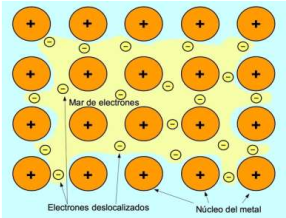
\includegraphics[width=5cm]{./imagenes/enlaceMetalico2.png} \end{center}
        \begin{itemize} 
            \item Elementos metálicos con baja energía de ionización.
            \item Unión entre núcleos atómicos y electrones de valencia.
        \end{itemize}
        \subsubsection{Propiedades}
            \begin{itemize}
                \item \textbf{Ductilidad:} tienen facilidad para formar hilos y poseen maleabilidad (capacidad para formar láminas) al aplicar presión.
                \item \textbf{Dureza:} son generalmente duros (resistentes al rayado).
                \item \textbf{Oxidación:} se oxidan con facilidad.
            \end{itemize}
            \begin{center} 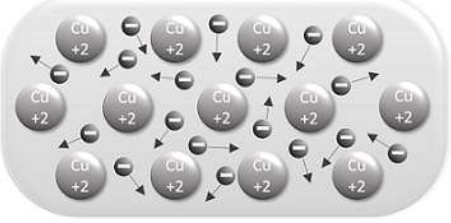
\includegraphics[width=5cm]{./imagenes/metalCu.png} \end{center}
            \begin{itemize}
                \item \textbf{Temperaturas de fusión y ebullición:} en metales son muy elevadas. Son sólidos a temperatura ambiente (excepto el mercurio, que es líquido).
                \item \textbf{Insolubles en agua:} en estado fundido son muy solubles en otros metales formando aleaciones.
                \item \textbf{Conductividad eléctrica:} buenos conductores de la electricidad (nube de electrones des-localizada) y del calor (facilidad de movimiento de electrones y de vibración de los restos atómicos positivos). La conductividad es mayor a bajas temperaturas.
            \end{itemize}
            \begin{center} 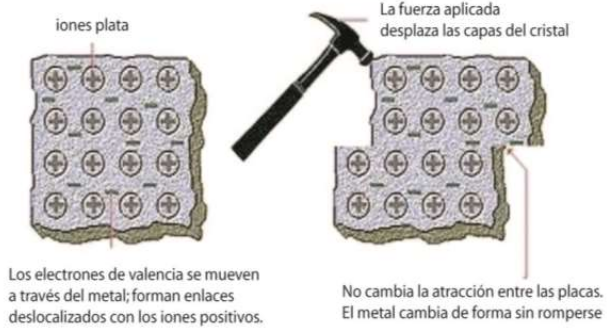
\includegraphics[width=7cm]{./imagenes/propiedadesMetal.png} \end{center}
        
    \subsection{Atracciones moleculares}
        \begin{center} 
            \begin{tabular}{| c | c |}
                \toprule
                \textbf{fuerzas} & \textbf{fuerzas} \\
                \textbf{inter-moleculares} & \textbf{intra-moleculares} \\
                \midrule
                Son las fuerzas de atracción & Son las fuerzas que  \\ 
                que existen entre moléculas. & mantienen juntos los \\
                                             & átomos de una molécula. \\
                \midrule
            \end{tabular}
        \end{center}
        \sangria{} Generalmente, las fuerzas inter-molecularess son mucho más débiles que las fuerzas intra-moleculares:
        \saltoPag{}
        \begin{center}
            \begin{tabular}{| c | c |}
                \toprule
                \textbf{fuerzas} & \textbf{fuerzas} \\
                \textbf{inter-moleculares} & \textbf{intra-moleculares} \\
                \midrule
                    $41 kJ$ para vaporizar & $930 kJ$ para romper todos \\
                    1 mol de agua.         & los enlaces $O-H$ en \\
                                           & 1 mol de agua. \\
                 \bottomrule
            \end{tabular}
        \end{center}
        \begin{center} \textbf{\underline{''Medidas'' de fuerzas inter-moleculares}} \end{center}
        \begin{itemize} 
            \item Punto de ebullición.
            \item Punto de fusión.
        \end{itemize}

        \begin{center} $\Delta H_{VAP}, \Delta H_{FUS}, \Delta H_{SUB}$ \end{center}
        \begin{center} \textcolor{blue}{\underline{Fuerzas de Van der Waals}} \end{center}
        \begin{itemize} 
            \item Dipolo-Dipolo.
            \item Fuerzas de dispersión.
            \item Puente de Hidrógeno.
        \end{itemize}
        \begin{center} \textcolor{blue}{\underline{Fuerzas electrostáticas}} \end{center}
        \begin{itemize}
            \item Ión-dipolo.
        \end{itemize}
        \subsubsection{Fuerza dipolo-dipolo}
            Existe entre moléculas polares, dado polares:
            \begin{center} $F = \frac{Q_1 Q_2}{d^2}$ \end{center}
            \begin{center}
                \begin{tabular}{| c |}
                    \toprule
                    Atracción electrostática de dos moléculas polares. \\
                    \bottomrule
                \end{tabular}
        \end{center}
            \begin{center} 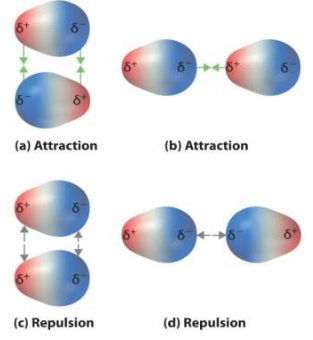
\includegraphics[width=4cm]{./imagenes/atraccionElectrostaticaDosMoleculasPolares.png} \end{center}
            \begin{center}
                \begin{tabular}{| c |}
                    \toprule
                    Interacción de muchos dipolos en \\ 
                    un estado condensado. \\
                    \bottomrule
                \end{tabular}
            \end{center}
            \begin{center} 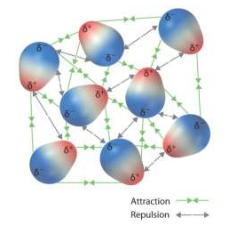
\includegraphics[width=4cm]{./imagenes/dipolosEnUnEstadoGaseoso.png} \end{center}
        \subsubsection{Fuerzas de dispersión}
            \begin{center} 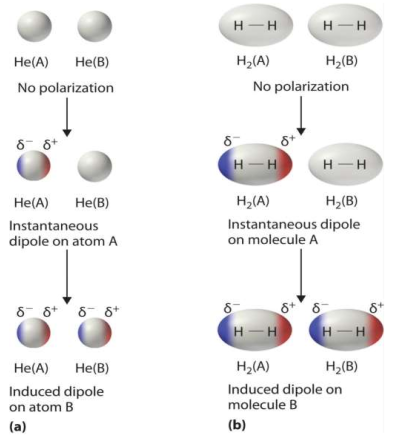
\includegraphics[width=7cm]{./imagenes/fuerzasDeDispersion.png} \end{center}
            \sangria{} Son fuerzas de atracción que surgen como resultado de dipolos temporales inducidos en átomos o moléculas. Están presentes en todas las moléculas. \\
            \sangria{} El carácter polarizable de los gases que contienen átomos o moléculas no polares, les permite condensarse. 
            \begin{center} \textbf{Ej:} $He, N_2, O_2, H_ 2$ \end{center}
            \sangria{} \textbf{Polarización} es la facilidad de distorsionar la distribución de los electrones en el átomo o molécula. \\
            \sangria{} La Polarización aumenta con:
            \begin{itemize}
                \item Mayor número de electrones, es decir, con la masa molar.
                \item Difusión de más nubes de electrones, es decir, con el área superficial de la molécula.
            \end{itemize}
            \begin{center} 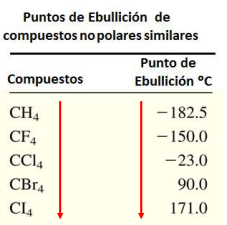
\includegraphics[width=6cm]{./imagenes/ebullicionDeCompuestosNoPolaresSimilares.png} \end{center}
        \subsubsection{Puente de Hidrógeno}
            \sangria{} El \textbf{enlace por puente de hidrógeno} es una interacción dipolo-dipolo especial entre el átomo de hidrógeno en un enlace polar $N-H$, $O-H$ o $F-H$ y un átomo electro-negativo de $O$, $N$ o $F$.
            \saltoPag{}
            \begin{center} \textcolor{blue}{\underline{Punte de hidrógeno: influencia}} \\[10pt] 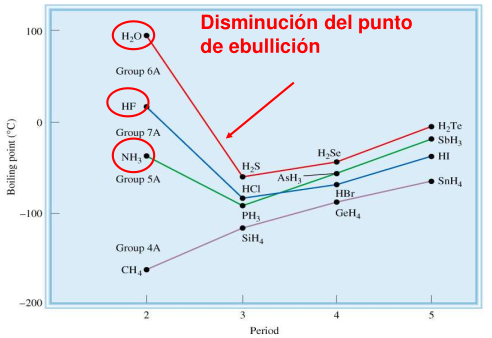
\includegraphics[width=8cm]{./imagenes/influenciaPuenteHidrogeno.png} \end{center}
            \begin{itemize}
                \item Estructuras de proteínas.
                \item Estructura de ácidos nucleicos.
                \item Propiedades anómalas del $H_2O$ (Peb, Pf, $\delta_{HIELO}$, propiedades disolventes, etc.)
            \end{itemize}
        \subsubsection{Interacción Ión-dipolo}
            \begin{itemize}
                \item Interacción entre un ión y un dipolo (Ej. $Na^+$ y $H_2O$).
                \item Es función de la carga y tamaño del ión y del momento dipolar y tamaño de la molécula.
            \end{itemize}
            \begin{center} 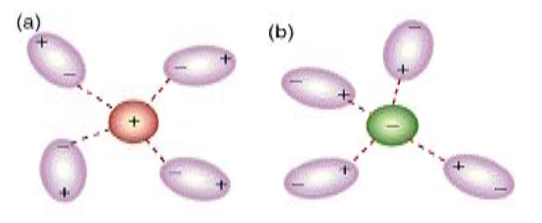
\includegraphics[width=6cm]{./imagenes/iteraccionIonDipolo.png} \end{center}
            \begin{center} \textbf{\underline{Ejemplo:}} interacción de una molécula de agua con un ión $Na^+$ y con un ión $Mg^{2+}$ \\[10pt] 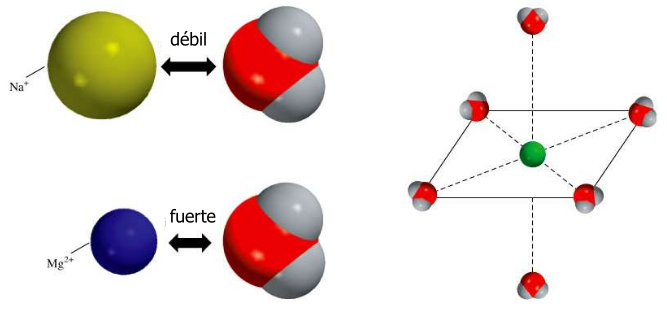
\includegraphics[width=8cm]{./imagenes/interaccionAguaNaMASMg2MAS.png} \end{center}
            

